\section{Theorien mit verborgenen Variablen und Bellsche Ungleichungen}
\label{sec:theorien_mit_verborgenen_variablen_bellsche_ungleichungen}


\subsection{Geschichte}
\label{subsec:geschichte}

Die Idee in der Wissenschaft, das Objekte, die weit voneinander entfernt sind, Auswirkungen auf einander haben können, geht schon auf Newton zurück - wenn nicht sogar weiter. Newton besagte mit seinem Newtonischen Gravitationsgesetz, dass alle Objekte sich gegenseitig anziehen, auch wenn sie in keinem direkten Kontakt stünden\footnote{\cite{newton_gravitation_2009}} . Michael Faraday und James Clerk Maxwell, die begründer der Feld-Theorie stellten die Vermutung auf, dass Elektromagnetismus
von einer Art ''Äther'' getragen werden könne, einer Art verborgenem Kraftfeld, was Anziehungs- und Abstoßkräfte übertrage\footnote{\cite{faraday_maxwell_ether}}. Die Idee das es Fremdwirkungen aus der Ferne geben könne und diese von verborgenen
Kräften, Medien oder Variablen übertragen werden, scheinen also nicht abwegig. Wie diese Ideen Einfluss auf die Diskussion um die Quantenverschränkung genommen haben, wird im folgenden erläutert. \\

\subsubsection{ERP-Paradoxon}
\label{subsubsec:erp_paradoxon}
Bevor das Phänomen der Quantenverschränkung bekannt war, gab es eine Diskussion darum, ob die Quantenmechanik eine Theorie ist, die die Realität vorllständig abbildet oder nicht.
Diese Diskussion an sich ist Bestandteil einer weitreichenderen Diskussion zwischen Niels Bohr und Albert Einstein,
die als Bohr-Einstein Debatte bekannt ist. Auf diese wird hier nicht im Detail eingegangen.\ Der Beginn des Diskussionsteils, auf den wir uns fokussieren,
ist die Veröffentlichung des nach den Autoren benannten EPR-Paradoxons von Albert Einstein, Boris Podolsky und Nathan Rosen. Darin argumentieren sie, dass die Quantenmechanik keine vollständige Theorie sein könne, da sie es erlaube
dass das Messen eines Partikels eine Fernwirkung auf ein anderes Partikel haben könne, unabhängig davon, wie weit die beiden Partikel voneinander entfernt seien\footnote{\cite{erp_1935}}. Es folgt ein Abriss der Argumentation von Einstein, Pdolsky und Rosen. \\\\
In dem Paper ''Can Quantum-Mechanical Description of Physical Reality Be Considered Complete?'' argumentieren Einstein, Podolsky und Rosen, dass
eine Theorie nur dann vollständig sein kann, wenn es zu jedem Element der physischen Realität ein Element in der Theorie gebe, was das Element
der physischen Realität abbilde/beschreibe.\\\\ Als 'Realität' definieren die Autoren das, was durch Experiment- und Messergebnisse bestimmt werden könne.
Dabei müssten diese Ergebnisse die Voraussetzung erfüllen, dass wenn man eine physikalische Menge genau bestimmen könnte, ohne ein System dabei zu stören,
dass es dann ein Element in der physikalischen Realität geben müsse, das dieser physikalischen Menge entspreche.\\\\
Das Argument der Autoren ist, dass die Quantenmechanik keine vollständige Abbildung der Realität liefere, da sie mit nicht kommutativen physikalischen Mengen arbeite.\
$AB \neq BA$ beute also, dass man keine nicht-probabilistische Aussage über die Eigenschaft B aussagen könne, wenn man den Wert für die Eigenschaft A kenne.\ Bringe man die Geschwindigkeit eines Partikels durch Messen in Erfahrung, könne man keine genaue Aussage mehr über die Position zum selben Zeitpunkt treffen,
da das Messen an sich den Zustand des Partikels ändere.\ Demnach könnten in der Welt der Quantenmechanik beide Eigenschaften, laut der im Artikel festgelegten Definition der Realität, nicht gleichzeitig existieren oder die Quantenmechanik liefere kein vollständiges Abbild der Realität.\\\\
Gleiches zeigen sie nochmal anhand einer Wellenfunktion, die zwei miteinander interagierende Systeme beschreibt.\ Beschreibt die Wellenfunktion den Zustand von zwei Partikeln X und Y und trennt die Partikel danach, könnte man laut der Quantenmechanik die Wellenfunktion dafür nutzen nach der Messung von einem der Partikel Aussagen über das andere Partikel zu treffen.\ Dabei müsse man sich allerdings entscheiden, für welche Eigenschaften man eine Messung durchführen möchte.\ Führt man die Messung für die Eigenschaft $A_X$ auf dem Partikel X aus, verändere man den Zustand von diesem Partikel und man könne keine Aussage mehr über die Eigenschaft $B_X$ treffen.\ Vor der Messung bestünde die Möglichkeit Formeln für beide Eigenschaften $A_Y$ und $B_Y$ für Partikel Y aufzustellen, um sie in Abhängigkeit von den Eigenschaften von Partikel X zu beschreiben, da sie vor der Trennung von der gleichen Wellenfunktion beschrieben werden konnten. Führt man die Messung von der Eigenschaft $A_X$ vom Partikel X aus, führe es deshalb dazu, dass die Eigenschaft $B_Y$ auch vom Partikel Y nicht mehr messbar werde. Man schreibe also Partikel Y die Realität der Eigenschaft $B_Y$ ab, obwohl man nur Partikel X gemessen hätte.\ Dieser Widerspruch führe zur Schlussfolgerung, dass die Quantenmechanik keine vollständige Theorie sei.\ Einstein und die anderen waren überzeugt, dass es eine Formulierung der Quantenmechanik geben müsse, die es erlauben würde, beide Eigenschaften gleichzeitig in Erfahrung zu bringen.\footnote{\cite{erp_1935}}
\ Dies führte dazu, dass etliche Theorien mit verborgenen Variablen formuliert wurden.\footnote{\cite{sep-qm-copenhagen}} \\

\subsubsection{Reaktion von Niels Bohr}
\label{subsubsec:reaktion_von_niels_bohr}
Bevor wir eine dieser Theorien mit verborgenen Variablen genauer betrachten, gehen wir noch kurz auf die Reaktion von Niels Bohr ein, der maßgeblich an der Entwicklung der Quantenmechanik beteiligt war.\\
In seinem Paper, mit dem gleichen Titel von Einstein, Podolsky und Rosen, widerspricht er der Definition von Realität, die die Autoren für ihre Argumentation genutzt haben.\ Eine Messung zu vollziehen
ohne das System zu verändern, sei laut ihm in der Quantenmechanik nicht möglich, da das Messinstrument in der Atomphysik im Gegensatz zur klassischen Physik mit dem beobachteten System interagieren müsse.\
Zudem stellt er infrage, ob es notwendig sei, sämtliche Kenngrößen in einer Messung festzustellen, da ein Experiment, das dafür aufgebaut wurde, um die Geschwindigkeit eines Partikels zu messen, eben nur für diesen Zweck
existiere und keinem anderem.\ Demnach wäre es unsinnig eine Beschreibung zu fordern, die sämtliche Eigenschaften eines Systems gleichzeitig beschreiben könne.\footnote{\cite{bohr_1935}}\\
Dies ist nur eine sehr vereinfachte Wiedergabe der beiden Ansichten von Einstein und Bohr.\ Da die Diskussion über die Mathematik der Quantenmechanik hinaus in Richtung philosophischer Fragen geht, was denn Realität sei und wie die Wissenschaft sie abbildet, ist dies eine Diskussion, die noch heute andauert.\\
Wie bereits erwähnt, gab und gibt es Wissenschaftler, die die Ansicht von Einstein, Podolsky und Rosen teilten und versuchten verborgene Variablen zu finden, die erklären, warum das Messen von einem System ein anderes, getrenntes System beeinflussen kann.\\

\subsubsection{Bohmsche Mechanik}
\label{subsubsec:bohmsche_mechanik}
Eine bekannte Theorie mit verborgenen Variablen ist die von Davod Bohm 1951. In seinen Artikeln ''A Suggested Interpretation of the Quantum Theory in Terms of ''Hidden'' Variables.''  behauptet Bohm eine Möglichkeit gefunden zu haben, unendlich präzise messen zu können, was der Heisenbergschen Unschärferelation widerspreche. Außerdem behauptet er in Form der Wellenfunktion, die er $\psi$-Feld nennt, eine Antwort auf das Paradoxon zu haben, was Einstein Podolsky und Rosen aufgestellt haben.\footnote{\cite{PhysRev.85.166}}\\
Bohms These beruht darauf, dass es ein sogenanntes $\psi$-Feld gäbe, das Einfluss auf Partikel nehme, aber selbst nicht von diesen beeinflusst werde und zudem nicht messbar sei. \\
Das $\psi$-Feld unterlege drei Kriterien:\\
1. dass es die Schrödingergleichung erfülle\\
2. dass wenn $\psi=R exp(is/\hbar)$ gelte, die Geschwindikeit eines Partikels auf $p=\nabla S(x)$ beschränkt sei und \\
3. dass die Wahrscheinlichkeitsverteilung der Position eines Partikels $P=|\psi(x)|^2$ sei. \\
Das $\psi$-Feld bestimme also zu jeder Zeit die Geschwindigkeit und Position eines Partikels. Da man das $\psi$-Feld noch nicht messen könne, könne man die genaue Positionen und Geschwindigkeiten von Partikeln nicht ermitteln.
In der klassischen Quantenmechanik messe man bisher nur Observablen von Partikeln, nicht aber das Partikel selbst. Er behauptet, dass die Messung einer Observablen unweigerlich zu kurzen, heftigen Schwingungen im umliegenden $\psi$-Feld führen würde.\\
Diese Schwingung im $\psi$-Feld sorgen dafür, dass ein Messergebnis kaum vorherzusagen sei, weil das $\psi$-Feld direkten Einfluss auf die Geschwindigkeit und Position eines Partikels habe. \\\\
Ein Messergebnis hinge laut Bohm von der initialen Position des zu messenden Objekts, sowie der initialen Form der Wellenfunktion, als auch vom Messapparat ab. Wenn man also die initiale Position und Geschwindigkeit eines Partikels, sowie die initiale Form der Wellenfunktion vor der Messung kennen würde und die Messung mit denselben initialen Zuständen wiederholen könnte, würde man beim Messen immer auf dasselbe Messergebnis stoßen. Die Messung müsste also deterministisch sein, wenn man alle Variablen kenne. Dafür wäre es allerdings notwendig, die tatsächliche Geschwindigkeit und Position eines Partikels zu kennen und nicht die Ergebnisse, die eine Observable liefern. Observablen liefern laut Bohm keine Informationen über das Partikel vor oder nach der Messung und würden vom Messapparat beeinflusst. Dies sorge auch dafür, dass die Messung einer Observablen der Eigenschaft Q, die nicht kommutativ mit der Eigenschaft P ist, die Observable derartig verändern würde, dass keine Aussage mehr über die Eigenschaft P getroffen werden könne. Beispielsweise könne keine Aussage mehr über die Geschwindigkeit eines Partikels getroffen werden, wenn dessen Position gemessen wurde.\\\\
Bohms Vorschlag einer Messung beider Werte gleichzeitig stellt er in folgendem Gedankenexperiment dar:\\
Wenn man ein erregtes Partikel zwischen zwei undurchlässigen, perfekt spiegelnden Wänden halten würde, sorge das $\psi$-Feld dafür, dass es zwischen den Wänden ruhe. Die gesamte kinetische Energie des Partikels würde in potenzielle/latente Energie umgewandelt werden. Messe man das Partikel in der Observable, die die Geschwindigkeit bestimmt, würde diese Energie wieder in kinetische Energie umgewandelt werden. Nehme man die Spiegel dann plötzlich und schnell genug weg, würde die kinetische Energie dafür sorgen, dass das Partikel irgendwo hinfliege. Messe man nach einer Weile die Distanz, die das Partikel geflogen ist und teile sie durch die Reisezeit, die mit dem Entfernen der Spiegelwände begonnen habe, könnte man die tatsächliche Geschwindigkeit des Partikels berechnen. \\Allerdings würde die Geschwindigkeit durch das Entfernen der Spiegel beeinflusst werden, da das Entfernen der Spiegel Wellenpakete im $\psi$-Feld  generieren würde. Durch die Kollision mit diesen Wellenpaketen könnte man allerdings auch bestimmen, in welchen der zwei Richtungen sich das Partikel bewegt habe. Dies Form der Messung der Bewegungsrichtung sei notwendig, da die Fluktuation des $\psi$-Feld derartig kompliziert sei, dass man nur zu einer Wahrscheinlichkeit aussagen könne, wohin das $\psi$-Feld ein Partikel bewege.
\\\\
Daraufhin geht er auf das EPR Paradoxon von Einstein Podolsky und Rosen ein. Einstein und die anderen gingen davon aus, dass die Quantenmechanik keine vollständige Theorie sei, da sie nicht erkläre, weshalb man mit einem Messergebnis eines Partikels, das in der Vergangenheit mit einem anderen Partikel interagiert habe, aussagen über das andere Partikel treffen könne, egal wie weit sie zum Zeitpunkt der Messung von einander entfernt seien und gleichzeitig nicht mehr ermöglicht Aussagen über das zweite Partikel zu treffen, die nicht gemessen wurden. Bohm behauptet, dass das Messen eines Partikels Fluktuationen im $\psi$-Feld um das Partikel verursache und schließt daraus, dass das $\psi$-Feld um das andere Partikel herum ähnlichen Fluktuationen unterliegen müsse. Damit wäre das $\psi$-Feld ein Medium zur Übertragung der Fluktuation oder genauer gesagt der Information, dass das erste Partikel gemessen wurde. Das $\psi$-Feld wäre dementsprechend das neue Limit für die Geschwindigkeit mit der Informationen übertragen werden können. Damit Stünde seine Theorie nicht mehr im Widerspruch zur Relativitätstheorie.\\\\
Die herkömmliche Interpretation der Quanteninformatik sage aus, dass man aufgeben müsse ein System mit einem präzisen Modell abzubilden, also die Unbestimmtheitsrelation als festen Bestandteil sehen zu müssen. Die Theorie von Bohm widerspreche dieser Aussage indem sie behaupte dass man Partikel und das umliegende $\psi$-Feld präzise beschreiben könne. So wie Forscher sich mit dem Atom beschäftigt haben, obwohl noch nie eins beobachtet wurde, solle man sich mit dem $\psi$-Feld auseinandersetzen und forschen, um es eines Tages berechnen oder gar messen zu können.
Obwohl Bohms Theorie auf viel Kritik stieß, da sie auf dem $\psi$-Feld als eine nicht messbare, nicht lokale, universelle Kraft beruhte, war sie ein gutes Beispiel dafür, dass Theorien mit verborgenen Variablen das Prinzip der Lokalität verletzen müssen. 1964 bewies John Stewart Bell dies mit der Bellschen Ungelichung.


\subsection{Bell`s Inequalität}
\label{subsec:bells_inequality}
Bell`s Inequalität bezieht sich auf die statistische Korrelation zwischen Messungen von verschränkten Teilchen.
Die Ungleichung wurde von John Bell 1964\footnote{\cite{bell_einstein_1964}} formuliert und besagt, dass die Wahrscheinlichkeit der Messergebnisse von verschränkten Teilchen durch eine lokale versteckte Variable erklärt werden können und hierdurch begrenzt ist.
Wenn die Korrelation jedoch über die Grenze der Ungleichung hinaus geht, kann dies nur durch Quantenmechanik erklärt werden.\\

Bell setzte für seine Idee voraus, mehrere Kopien von verschränkten Teilchen zu haben. Dise Partikel können heutzutage druch ein Zerfallsprozess erreicht werden in dem ein Partikel in zwei verschränkte Teilchen zerfällt.\\

Durch den Zerafll eines Teilchen und dem Stern-Gerlach-Experiment wissen wir, dass ein Teilchen mit einem Spin von 0 in zwei Teilchen mit einem Spin von 1/2 zerfällt.
\begin{equation}
    S = 0 \rightarrow S_1 = S_2 = \pm\frac{1}{2}
\end{equation}
Beide Teilchen haben den Spin von $\pm\frac{1}{2}$, müssen jedoch sich gegenseitig aufheben, so dass die Summe der Spins 0 ergibt.
Dies nennt man auch Spin up und Spin down. Wenn das eine Teilchen Spin up ist, muss das andere Spin down sein und anders herum.\\
Dadurch sind die beide Teilchen miteinander verschränkt und kann wie folgt beschrieben werden:
\begin{equation}
    \ket{\psi} = \frac{1}{\sqrt{2}}(\ket{\uparrow}\ket{\downarrow} - \ket{\downarrow}\ket{\uparrow})
\end{equation}

Gehen wir davon aus, dass wir zwei Messungen durchführen. Die Messung von Alice und die Messung von Bob.
Beide dürfen den Spin des Partikels in jede beliebige Richtung messen. Wie sind die beiden Messungen korreliert?\\
Laut Einstein ist jedes einzelne Teilchen deterministisch. Das bedeutet, dass die Messung vom Spin des Teilchens nicht zufällig ist, sondern durch eine versteckte Variable bestimmt wird und dadurch der Spin beider Teilchen nicht korreliert ist.\\
Daraus folgernd müssen die Messergebnisse deterministisch sein. Wenn Bob $(+a, +b, -c)$ misst, dann muss Alice $(-a, -b, +c)$ sein, welches durch die versteckte Variable vorherbestimmt ist und zusammen ein 0 Spin ergibt.
Durch die Voraussetzung des Aufheben des Spins kann eine Tabelle von allen deterministischen Messergebnissen erstellt werden.

\begin{figure}[H]
    \centering
    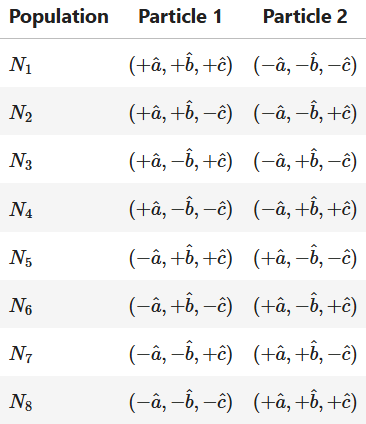
\includegraphics[width=0.5\linewidth]{img/BellList.png}
    \caption{Bell zuständen nach der versteckten Variable}
    \label{fig:BellList}
\end{figure}

Jetzt errechnen wir die Wahrscheinlichkeit, dass Alice und Bob bei unabhängigen Messungen dasselbe Vorzeichen messen. Die Wahrscheinlichkeit in Zeile 1 und 8 sind $0\%$und in Zeile 2 bis 7 sind es $P = \frac{4}{9}$.
Das bedeutet nach Einstein die Wahrscheinlichkeit, dass Alice und Bob dasselbe messen $P \leq \frac{4}{9}$ ist. Dies ist Bell`s Inequalität.\\
Vorliegendes Beispiel ist generalisiert und kann auf beliebige Winkel angewendet werden, wobei die Wahrscheinlichkeit wie folgt für alle möglichen Winkel berechnet wird.
\begin{equation}
    E(\overrightarrow{a}, \overrightarrow{b}) = \int d\lambda \rho(\lambda) A(\overrightarrow{a}, \lambda) B(\overrightarrow{b}, \lambda)
\end{equation}

Nun zu der Wahrscheinlichkeit nach der Quantenmechanik. Wir gehen davon aus, dass Bob den Spin in $a$ Richtung misst, Beispielsweise spin up. Daraus folgernd muss, wenn Alice in $a$ Richtung misst, das Ergebniss Spin down sein.\\
Dadurch, dass wir das Ergebniss einer der Achsen kennen, können wir die Wahrscheinlichkeit für die anderen Achsen mit folgender Gleichung berechnen.
\begin{equation}
    P(b) = \cos^2(\frac{\theta}{2})
\end{equation}
Hierbei ist $\theta$ der Winkel zwischen den Achsen. Wenden wir dies auf das Beispiel auf die Achse $b$ an so setzen wir $\theta = 60^\circ$
\begin{equation}
    P(b) = \cos^2(\frac{60^\circ}{2}) = \frac{3}{4}
\end{equation}
Machen wir dies auch für die andere Achse $c$ wo $\theta = 120^\circ$ ist erhalten wir
\begin{equation}
    P(c) = \cos^2(\frac{120^\circ}{2}) = \frac{1}{4}
\end{equation}
Von diesen beiden Wahrscheinlichkeit errechnen wir den Durchschnitt von $P = \frac{1}{2}$, was bedeutet das Bell`s Inequalität mit $P = \frac{1}{2} \ge \frac{4}{9}$ verletzt ist.\\

\subsubsection{Bell im Quantumcomputer}
\label{subsubsec:bell_quantumcomputer}
Wir haben das Beispiel von Bell`s Inequalität in der Quantenmechanik gezeigt, jedoch ist es auch möglich dies in einem Quantumcomputer zu zeigen.
Hierbei haben wir das Bells Theorem folgendermaßen umgesetzt\footnote{\cite{qiskit_entanglement_2024}}.
\begin{figure}[H]
    \centering
    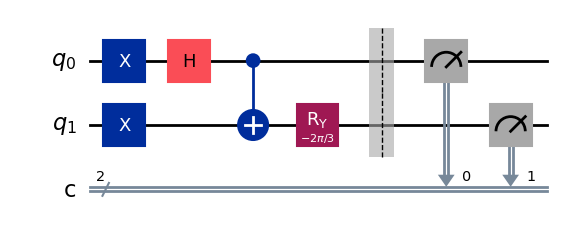
\includegraphics[width=0.9\linewidth]{img/BellCircuit.png}
    \caption{Bell`s Theorem im Quantumcomputer}
    \label{fig:BellCircuit}
\end{figure}

Die beiden Linien $q_0$ und $q_1$ sind die beiden verschränkten Teilchen, die durch den Zerfall eines Teilchens entstanden sind.
Den verschänkten Zustand erreichen wir durch die beiden $X$ gates, das $H$ gate und das CNOT gate.
Nachdem wir den verschränkten Zustand erreicht haben, messen wir $q_0$ in der $a$ Achse und $q_1$ an der $b$ Achse. Dies ist mit dem $R_y$ gate realisiert der die Messung um $120^\circ$ dreht.\\

Um eine genaueres Ergebniss zu erhalten, führen wir diese Messungen 30000 mal durch
\begin{figure}[H]
    \centering
    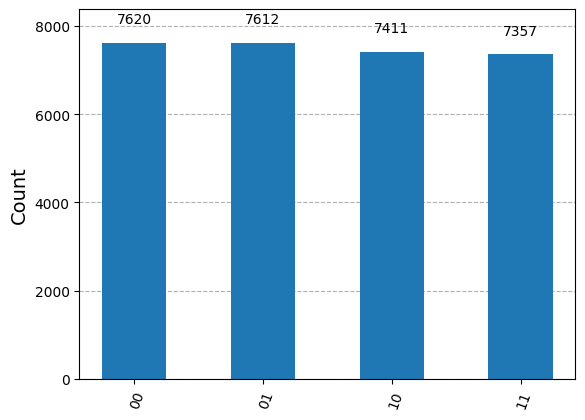
\includegraphics[width=0.8\linewidth]{img/BellResult.png}
    \caption{Ergebniss von Bell`s Theorem im Quantumcomputer}
    \label{fig:BellResult}
\end{figure}

Die Ergebnisse zeigen das die Wahrscheinlichkeit dasselbe Vorzeichen zu messen bei $P = (7620 + 7357) / 30000 = 0.49923$ oder auch 49,923\% liegt, was Bell`s Inequalität verletzt.\\


\subsection{CHSH Game}
\label{subsec:chsh_experimentell}
Das CHSH Spiel basiert auf einem Gedankenexperiment und ist eine Alternative Erklärung für die Verletzung der Bell`s Inequalität.\\
Das Gedankenexperiment wurde von John Clauser, Michael Horne, Abner Shimony und Richard Holt 1969\footnote{\cite{clauser_proposed_1969}} kurz nach der Veröffentlichung von Bell`s Inequalität vorgeschlagen.\\

In diesem Abschnitt werden wir das CHSH Spiel erklären und wie es in einem Quantumcomputer umgesetzt werden kann.\\

\subsubsection{Nonlocal Games}
\label{subsubsec:chsh_nonlocal}

Um die Grundlagen des Spieles zu verstehen müssen wir zuerst erklären was ein \textbf{Nonlocal Game} ist unter welches das CHSH Spiel fällt.
\begin{enumerate}
    \item Das Spiel wird von zwei Spielern gespielt, Alice und Bob, die in Kooperation zusammenarbeiten. Das bedeutet, dass beide Spieler zusammen gewinnen oder verlieren.
    \item Ein Schiedsrichter leitet das Spiel, indem er den Spielern Fragen stellt und anschließend ihre Antworten überprüft und mitteilt, ob die Spieler gewonnen oder verloren haben.
    \item Nachdem die Spieler die Frage vom Schiedsrichter erhalten haben, dürfen beide Spieler nicht mehr miteinander kommunizieren. Vorherige Absprachen und Taktiken sind erlaubt.
\end{enumerate}

\begin{figure}[H]
    \centering
    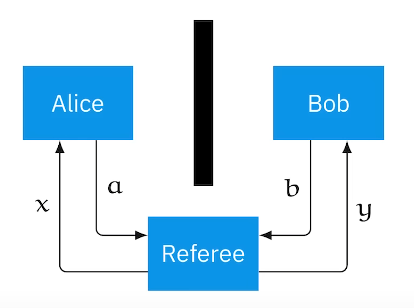
\includegraphics[width=0.6\linewidth]{img/CHSH-drawing.png}
    \caption{CHSH Spielaufbau \protect\cite[47m20s]{IBM_chsh_2025}}
    \label{fig:CHSHGame}
\end{figure}

Sowohl die beiden Fragen $x$ und $y$ als auch die Antworten $a$ und $b$ können beliebige Werte annehmen. In unserem Fall werden alle Fragen und Antworten als binäre Bits dargestellt.\\

Um den Spielverlauf zu verstehen, betrachen wir den Schiedsrichter nun etwas genauer und welche aufgaben er hat.
\begin{enumerate}
    \item Der Schiedsrichter stellt die Fragen $x$ und $y$ zufällig, in unserem Fall $x, y \in \{0, 1\}$.
    \item Alice und Bob antworten mit den Antworten $(a, b)$. Wobei sie durch die fehlende Kommunikation nicht wissen, welche Frage der andere Spieler gestellt bekommen hat oder wie dieser geantwortet hat.
    \item Der Schiedsrichter überprüft die Antworten $(a, b)$ bezogen auf die gestellten Fragen $(x, y)$ und entscheidet nach einer festgelegten Regel, ob die Spieler gewonnen oder verloren haben.
    \item Beide Spieler kennen die Regel, nach der der Schiedsrichter entscheidet, ob sie gewonnen oder verloren haben.
\end{enumerate}

Durch die Beschreibung des Schiedsrichters erhalten wir verschiedene Arten von \textbf{Nonlocal Games} wie das CHSH Spiel.\\

\subsubsection{CHSH Definition}
\label{subsubsec:chsh_definition}

Nun definieren wir den Schiedsrichter für das CHSH Spiel.
\begin{enumerate}
    \item Alle Fragen und Antworten sind binäre Bits.
    \begin{equation}
        x, y, a, b \in \{0, 1\}
    \end{equation}
    \item Alle Fragen werden zufällig gestellt.
    \item Ein paar von Antworten $(a, b)$ gewinnt für $(x, y)$, wenn
    \begin{equation}
        a \oplus b = x \land y
    \end{equation}
    und verliert wenn es nicht so ist.
    \begin{table}[H]
        \centering
        \begin{tabular}{c|c}
            $(x, y)$ & Gewinnbedingung \\ \hline
            $(0, 0)$ & $a = b$ \\ \hline
            $(0, 1)$ & $a = b$ \\ \hline
            $(1, 0)$ & $a = b$ \\ \hline
            $(1, 1)$ & $a \neq b$ \\
        \end{tabular}
        \caption{Gewinnbedingung für alle möglichen Fragen}
        \label{tab:CHSHWinCondition}
    \end{table}
\end{enumerate}

\subsubsection{Taktiken für das CHSH Spiel}
\label{subsubsec:chsh_taktiken}

Mit diesen Gewinnbedingungen können wir nun verschiedene Taktiken für das CHSH Spiel definieren.
Wie zuvor bei der Bell Inequalität fangen wir mit der klassischen Taktik an und gehen dann zur Quantentaktik über.\\

\textbf{Klassische Taktik}
Die Klassische herangehensweie ist die deterministische Taktik mit welcher es nicht möglich ist in allen fällen zu gewinnen.
\begin{align}
    a(0) \oplus b(0) &= 0 \\
    a(1) \oplus b(0) &= 0 \\
    a(0) \oplus b(1) &= 0 \\
    a(1) \oplus b(1) &= 1
\end{align}

Aus dieser Erkentniss können wir die beste Gewinnwahrscheinlichkeit ablesen.
Diese beträgt $P = \frac{3}{4}$ und ist recht einfach zu erreichen wenn Alice und Bob auf egal welche Frage immer mit $0$ antworten\\

Eine ähnliche Taktik ist die probabilistische Taktik, jedoch ist die Gewinnwahrscheinlichkeit hierbei die selbe wie bei der deterministischen Taktik.
Das hat den Grund das eine probabilistische Taktik als eine zufallswahl eine deterministische Taktik gewertet werden kann und dadurch den selben Effekt erzielt.\\

\textbf{Quantentaktik}
Um zu beweisen das der Quantenmechanische Ansatz besser ist als der klassische Ansatz, müssen wir die Gewinnwahrscheinlichkeit berechnen.\\

Zuerst definieren wir ein Einheitsvektor für alle Winkel $\theta$ (In Rad).
\begin{equation}
    \ket{\psi_\theta} = \cos(\theta) \ket{0} + \sin(\theta) \ket{1}
\end{equation}

Außerdem definieren wir für den Einheitsvektor eine Unitäre Matrix $U(\theta)$ um $\psi_\theta$ an $\ket{0}$ und $\psi_{\theta+\pi/2}$ an $\ket{1}$ zu koppeln.
\begin{equation}
    U(\theta) = \ket{0}\bra{\psi_\theta} + \ket{1}\bra{\psi_{\theta+\pi/2}}
\end{equation}

Nun kommen die beiden verschränkten Teilchen ins Spiel.\\

Alice wendet nun die Unitäre Matrix wie folgt auf $a$ an.
\begin{equation}
    \begin{Bmatrix}
        U_\theta & \hbox{if} & x = 0 \\
        U_{\pi/4} & \hbox{if} & x = 1
    \end{Bmatrix}
\end{equation}

Zuletzt misst Alice $a$ und sendet das Ergebniss an den Schiedsrichter. Und Bob macht fast das selbe.
\begin{equation}
    \begin{Bmatrix}
        U_{\pi/8} & \hbox{if} & y = 0 \\
        U_{-\pi/8} & \hbox{if} & y = 1
    \end{Bmatrix}
\end{equation}
Wie diese angaben von $\theta$ zustande kommen, wird im nächsten Abschnitt erklärt.\\

Um nun die Gewinnwahrscheinlichkeit zu berechnen, nehmen wir eine der möglichen Fragen und berechnen die Wahrscheinlichkeit wie $(x, y) = (0, 0)$.\\
Das bedeutet Alice wendet $U_\theta$ an und Bob wendet $U_{\pi/8}$ an.\\

\begin{equation}
    (U_\theta \otimes U_{\pi/8})\ket{\phi^+} = \frac{\cos(-\frac{\pi}{8})\ket{00} + \cos(-\frac{5\pi}{8})\ket{01} + \cos(\frac{3\pi}{8})\ket{10} + \cos(-\frac{\pi}{8})\ket{11}}{\sqrt{2}}
\end{equation}

Die daraus entstehenden Wahrscheinlichkeiten sind

\begin{center}
    \begin{tabular}{c|c|c}
    $(a, b)$ & Wahrscheinlichkeit & Vereinfacht \\ \hline
    $(0, 0)$ & $\frac{1}{2}\cos^2(-\frac{\pi}{8})$ & $\frac{2+\sqrt{2}}{8}$ \\
    $(0, 1)$ & $\frac{1}{2}\cos^2(-\frac{5\pi}{8})$ & $\frac{2-\sqrt{2}}{8}$ \\
    $(1, 0)$ & $\frac{1}{2}\cos^2(\frac{3\pi}{8})$ & $\frac{2-\sqrt{2}}{8}$ \\
    $(1, 1)$ & $\frac{1}{2}\cos^2(-\frac{\pi}{8})$ & $\frac{2+\sqrt{2}}{8}$
    \end{tabular}
\end{center}

von diesen Wahrscheinlichkeiten interessiert uns welche davon gewinnen und verlieren. 
\begin{align}
    P_w(a = b) = \frac{2+\sqrt{2}}{4} \approx 0.85 \\
    P_l(a \neq b) = \frac{2-\sqrt{2}}{4} \approx 0.15
\end{align}
Für die anderen drei Fragen $(x, y) = (0, 1), (1, 0), (1, 1)$ sind die Wahrscheinlichkeiten die selben. Nur das bei $(1, 1)$ die Gewinnwahrscheinlichkeit $P_w(a \neq b)$ ist.\\
Der Durchschnitt aller Fragestellungen ergibt eine Gewinnwahrscheinlichkeit von $P = 0.85$ was bedeutet das die Quantentaktik besser ist als die klassische Taktik.\\

\textbf{Geometrische Interpretation}\\
Um besser zu veranschaulichen warum die Winkel von $\theta$ gewählt wurden, können wir dies geometrisch darstellen.\\
Dafür benutzen wir die vorherige Gleichung
\begin{equation}
    \braket{\psi_\alpha \oplus \psi_\beta | \phi^+} = \frac{1}{\sqrt{2}}\braket{\psi_\alpha | \psi_\beta}
\end{equation}

Dies stellt die Wahrscheinlichkeit der Antworten für die Frage $(x, y) = (0, 0)$ folgend dar\\

\begin{center}
    \begin{tabular}{c|c}
    $(a, b)$ & Wahrscheinlichkeit \\ \hline
    $(0, 0)$ & $\frac{1}{2}\lvert \braket{\psi_0 | \psi_\frac{\pi}{8}} \rvert^2$  \\
    $(0, 1)$ & $\frac{1}{2}\lvert \braket{\psi_0 | \psi_\frac{5\pi}{8}} \rvert^2$  \\
    $(1, 0)$ & $\frac{1}{2}\lvert \braket{\psi_\frac{\pi}{2} | \psi_\frac{\pi}{8}} \rvert^2$  \\
    $(1, 1)$ & $\frac{1}{2}\lvert \braket{\psi_\frac{\pi}{2} | \psi_\frac{5\pi}{8}} \rvert^2$
    \end{tabular}
\end{center}

\begin{figure}[H]
    \centering
    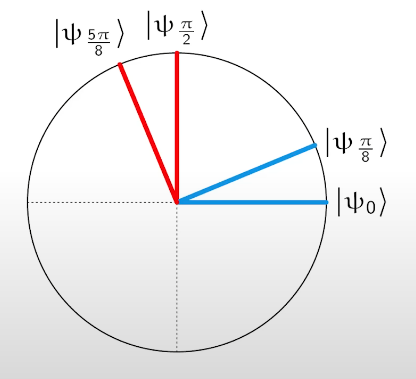
\includegraphics[width=0.6\linewidth]{img/CHSH-geometric.png}
    \caption{Geometrische Interpretation von $\theta$ \protect\cite[1h3m]{IBM_chsh_2025}}
    \label{fig:CHSHGeometric}
\end{figure}

Die Blauen Vektoren beschreiben die Wahrscheinlichkeit das, dass Ergebniss 0 ist und die Roten Vektoren das Ergebniss 1 ist.
Umso näher die Vektoren aneinander sind, desto höher ist die Wahrscheinlichkeit das die Antwort gleich ist.\\

Bei den anderen Fragestellungen ist die Darstellung ähnliche, nur bei der Frage $(1, 1)$ sind die Vektoren deutlich weiter auseinander.
Da wir bei dieser Frage eine unterscheidliche Antwort brauchen ist das aber genau das was wir wollen.\\

\subsubsection{CHSH im Quantumcomputer}
\label{subsubsec:chsh_quantumcomputer}
Wir haben das CHSH Spiel in einem Quantumcomputer umgesetzt und die Gewinnwahrscheinlichkeit berechnet.\\
Hierbei haben wir mit einem Estimator die Gewinnwahrscheinlichkeit aller Phasen berechnet und diese mit der klassischen Taktik verglichen\footnote{\cite{IBM_chsh_2025}}.

\begin{figure}[H]
    \centering
    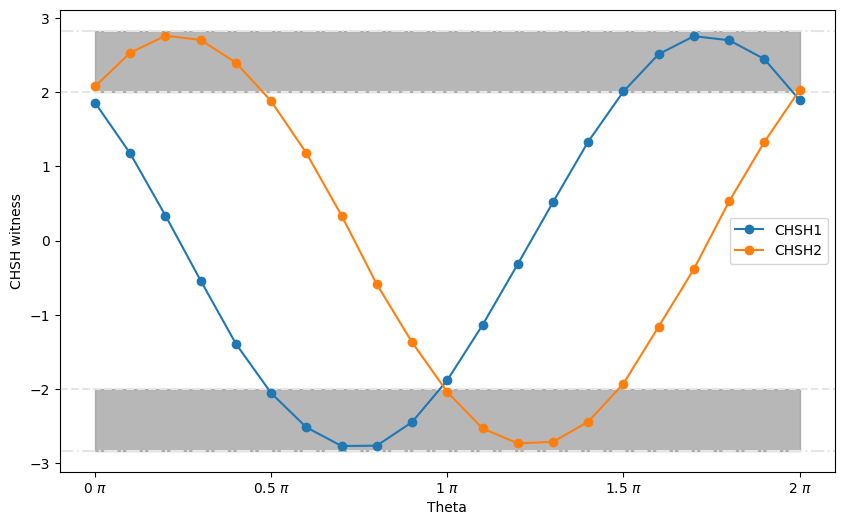
\includegraphics[width=0.8\linewidth]{img/CHSH-Output.png}
    \caption{CHSH Spiel im Quantumcomputer}
    \label{fig:CHSHQuantum}
\end{figure}

Der Weiße innere bereich ist der Bereich der mit klassischen Methoden erreicht werden kann.
Die beiden Linien zeigen die Wahrscheinlichkeit der Antworten $(a, b)$ für alle Fragen.\\
Mit Grau ist der Bereich markeirt der nur von Quantenmechanischen Methoden erreicht werden kann. Alles was darüber hinaus geht ist mit keiner bekannten methode zu erreichen.\\
